\chapter{ ARCHITECTURE }

Nous avons choisi une architecture dites "MVC", Modèle, Vue, Contrôleur. 
Ce choix a été fait dans un but de maintenabilité. En effet notre projet, et plus particulièrement le dépôt Github du projet est partagé avec le groupe 3. Notre code étant donc repris par d'autres développeurs, il est nécessaire que celui-ci soit clair et bien organisé pour leur permettre de modifier ou d'ajouter des fonctionnalités.
\\
\begin{figure}[H]
    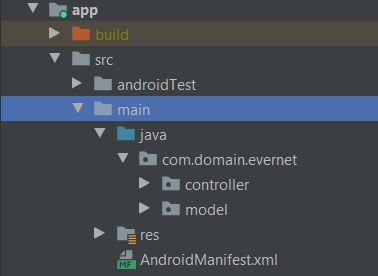
\includegraphics[width=10cm]{images/arbo.png}
    \caption{Arborescence de l'application Evernet.}
\end{figure}

\begin{itemize}
    \item [•] Modèle : \\
    Contient toutes les classes métiers nous permettant de traiter les données, ainsi que les communications.
    Cela inclut donc la communication avec le serveur central via Socket, les communications entre clients via SMS; la création de paquets; ainsi que le traitement des images. Ces fichiers sont accessibles dans le dossier model.
    \\
    
    \item [•] Vue \\
    Il s'agit ici de tous les fichiers XML permettant de construire l'interface utilisateur. Ces fichiers sont accessibles depuis le dossier res, les fichiers moteurs sont dans le dossier layout.
    \\
    
    \item [•] Contrôleur \\
    Cette partie contient toutes les classes activité et fragment qui permettent de faire le lien entre la vue et le modèle. La classe principale contrôlant le projet est MainActivity.
    Ces fichiers sont accessibles depuis le dossier controller.
    
\end{itemize}

\begin{figure}[H]
    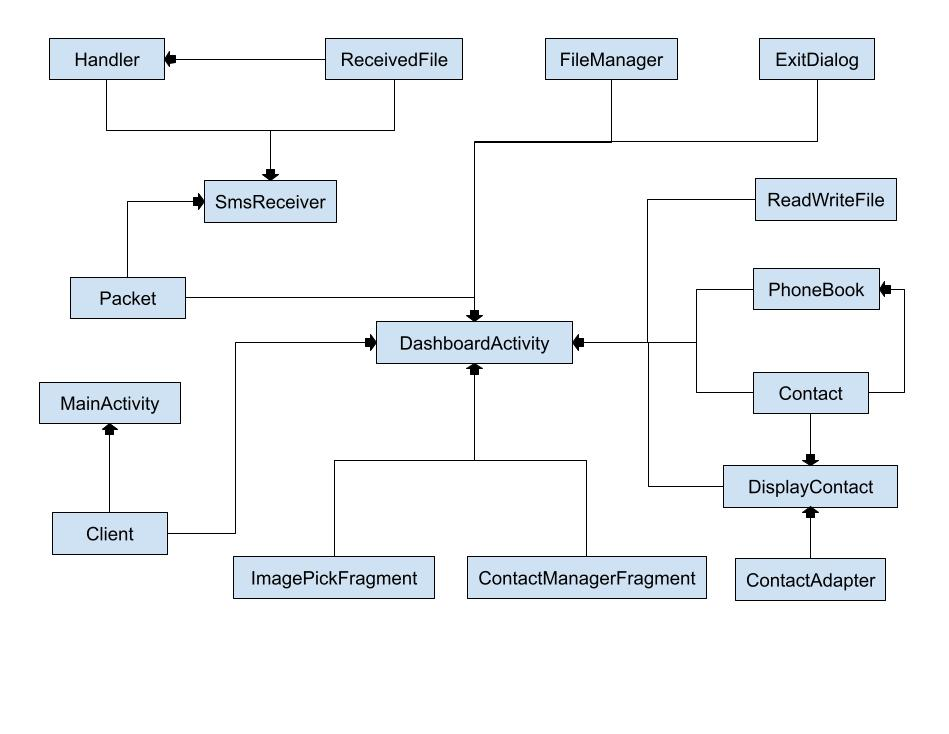
\includegraphics[width=15cm]{images/architecture.jpg}
    \caption{Diagramme de l'architecture.}
\end{figure}
